% AUTO-GENERATED by update_report_from_results.py -- do not edit by hand
\providecommand{\GeneratedForecastingFigures}{}
\renewcommand{\GeneratedForecastingFigures}{%
\begin{figure}[!htbp]
\centering

\includegraphics[width=0.72\linewidth]{figures/generated/horizon_mae.png}
\caption{Forecast error by horizon on the held-out test split. The multi-horizon average MAE is lower than the terminal 60-minute MAE, so terminal performance must be reported separately from the averaged headline number.}
\label{fig:horizon_mae}
\end{figure}
}
\providecommand{\GeneratedPersonalizationFigures}{}
\renewcommand{\GeneratedPersonalizationFigures}{%
\begin{figure}[!htbp]
\centering
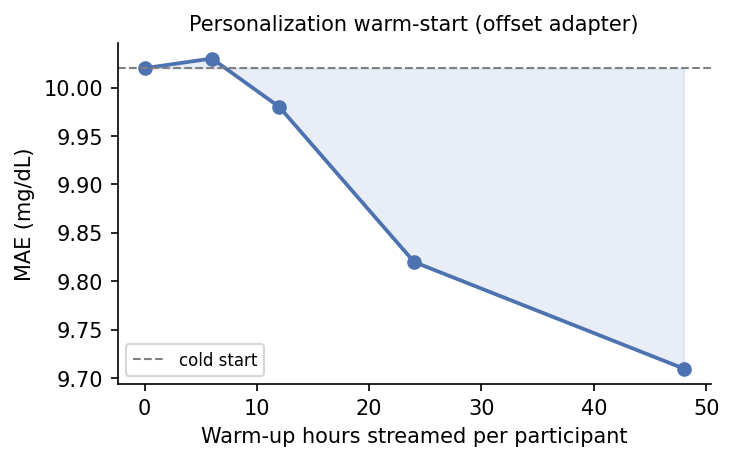
\includegraphics[width=0.68\linewidth]{figures/generated/personalization_warmup.png}
\caption{Warm-up sweep from the original evaluation. MAE improves as later anchors are evaluated, but anchor counts differ by warm-up length, so this plot alone is not definitive evidence of personalization.}
\label{fig:personalization_warmup}
\end{figure}
\begin{figure}[!htbp]
\centering
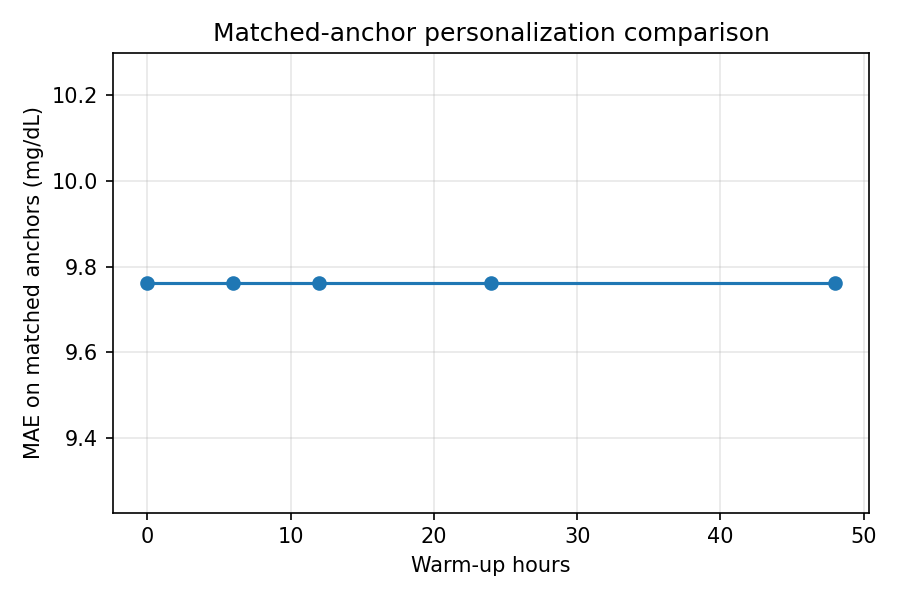
\includegraphics[width=0.68\linewidth]{figures/generated/personalization_matched_anchor.png}
\caption{Matched-anchor personalization diagnostic. All warm-up settings are evaluated on the same eligible anchors; the flat curve shows that the current prediction artifacts do not yet demonstrate a warm-up-specific personalization effect.}
\label{fig:personalization_matched_anchor}
\end{figure}
}
\providecommand{\GeneratedScenarioFigures}{}
\renewcommand{\GeneratedScenarioFigures}{%
\begin{figure}[!htbp]
\centering
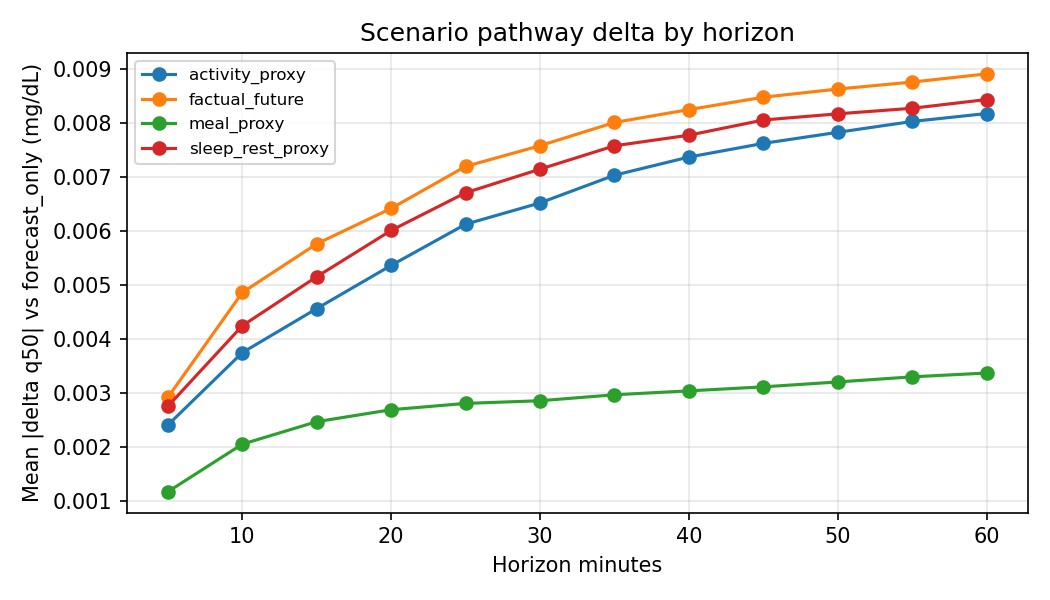
\includegraphics[width=0.75\linewidth]{figures/generated/scenario_delta_by_horizon.png}
\caption{Absolute prediction deltas between proxy scenario modes and forecast-only mode. Deltas are far below clinically meaningful mg/dL changes, indicating that the scenario pathway is currently inactive or weakly used.}
\label{fig:scenario_delta}
\end{figure}
}
\providecommand{\GeneratedSafetyFigures}{}
\renewcommand{\GeneratedSafetyFigures}{%
\begin{figure}[!htbp]
\centering
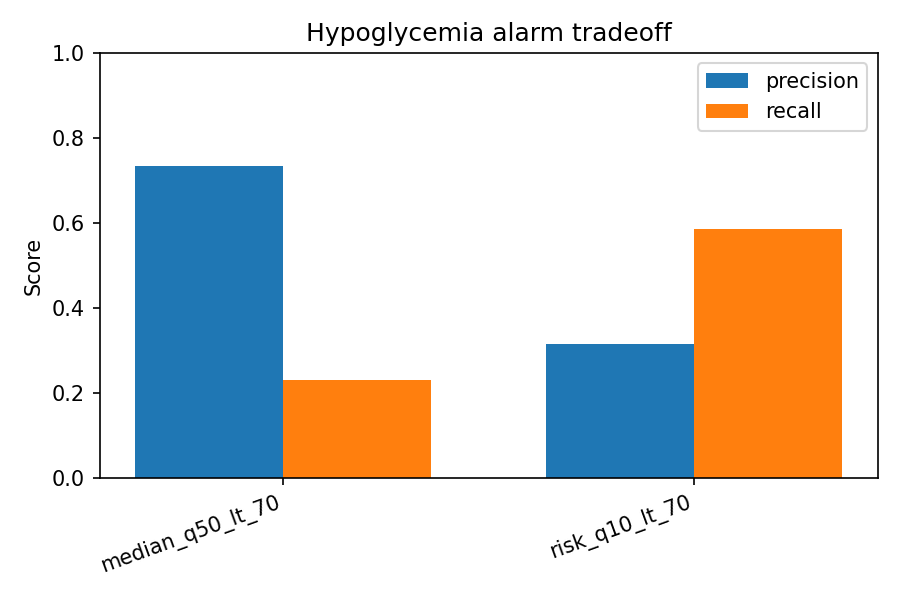
\includegraphics[width=0.72\linewidth]{figures/generated/hypo_alarm_tradeoff.png}
\caption{Clinical alarm trade-off. Median forecasts are conservative for hypoglycemia, while the q0.1 risk rule increases recall at the cost of lower precision.}
\label{fig:hypo_alarm_tradeoff}
\end{figure}
}
\providecommand{\GeneratedSubgroupFigures}{}
\renewcommand{\GeneratedSubgroupFigures}{%
\begin{figure}[!htbp]
\centering
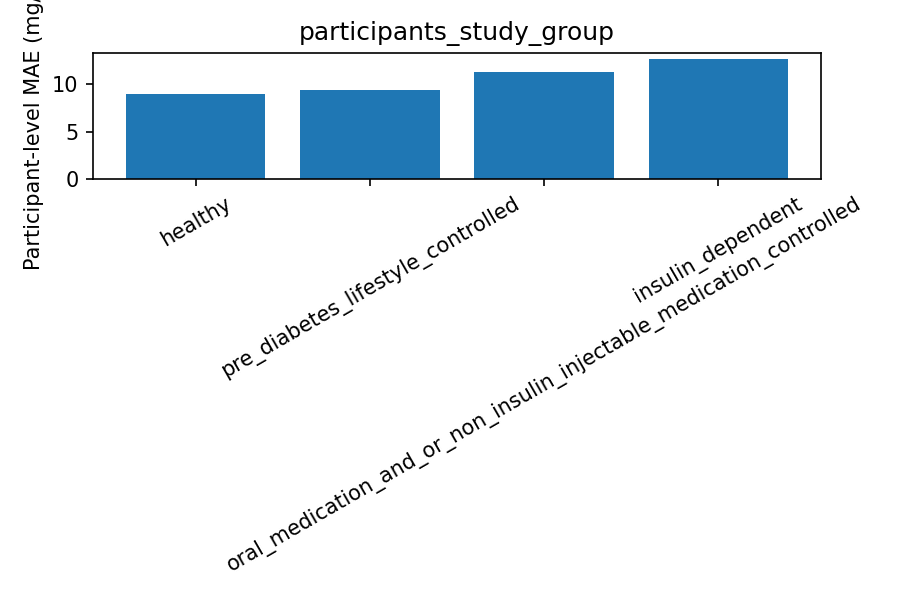
\includegraphics[width=0.82\linewidth]{figures/generated/subgroup_mae_study_group.png}
\caption{Participant-level MAE by AI-READI study group. Insulin-dependent and medication-treated groups are harder to forecast than healthy controls, consistent with higher glycemic variability.}
\label{fig:subgroup_study_group}
\end{figure}
\begin{figure}[!htbp]
\centering
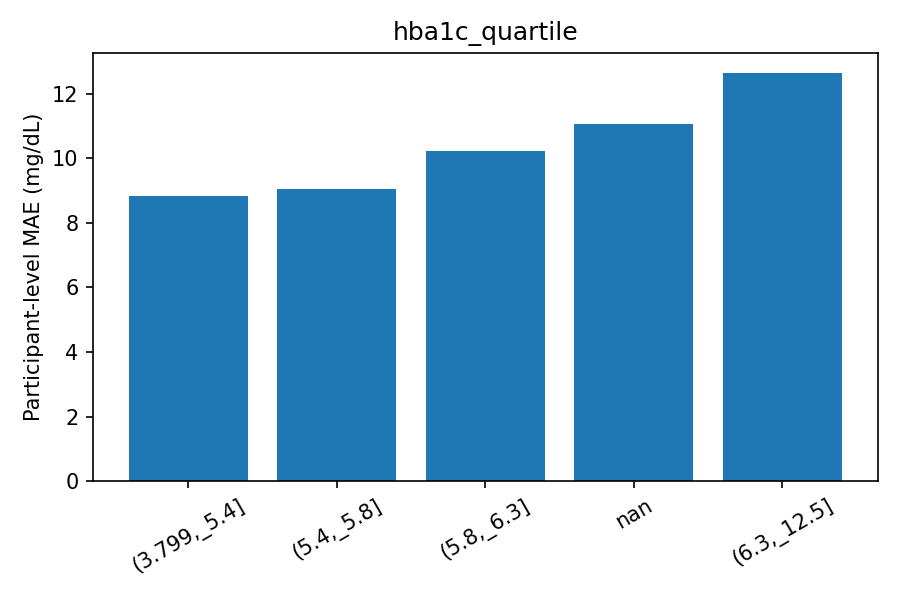
\includegraphics[width=0.82\linewidth]{figures/generated/subgroup_mae_hba1c.png}
\caption{Participant-level MAE by HbA1c quartile. Higher HbA1c strata show larger errors, supporting phenotype-level error analysis beyond a single aggregate MAE.}
\label{fig:subgroup_hba1c}
\end{figure}
\begin{figure}[!htbp]
\centering
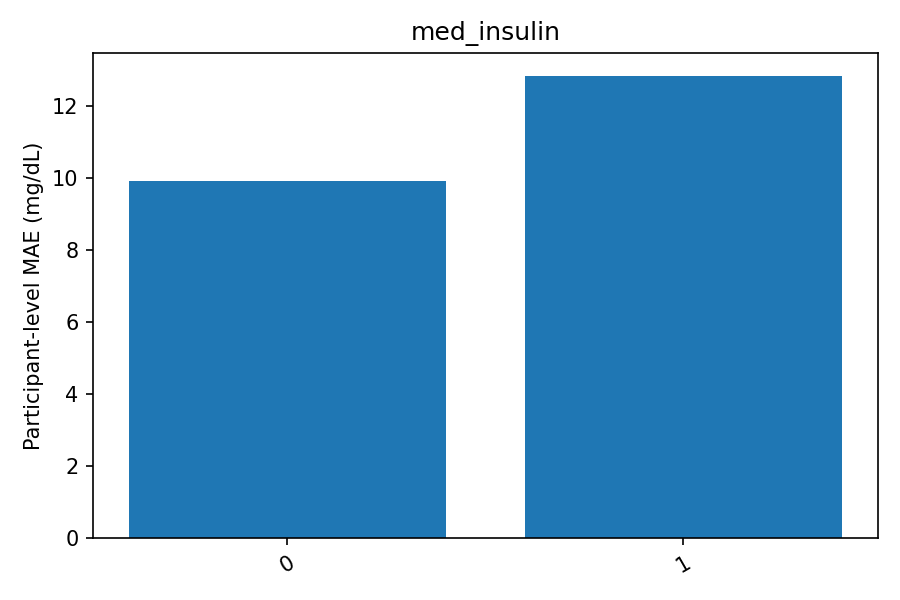
\includegraphics[width=0.82\linewidth]{figures/generated/subgroup_mae_med_insulin.png}
\caption{Participant-level MAE stratified by the static med\_insulin metadata flag. This is a therapy-status subgroup, not an insulin action or dose counterfactual.}
\label{fig:subgroup_med_insulin}
\end{figure}
\begin{figure}[!htbp]
\centering
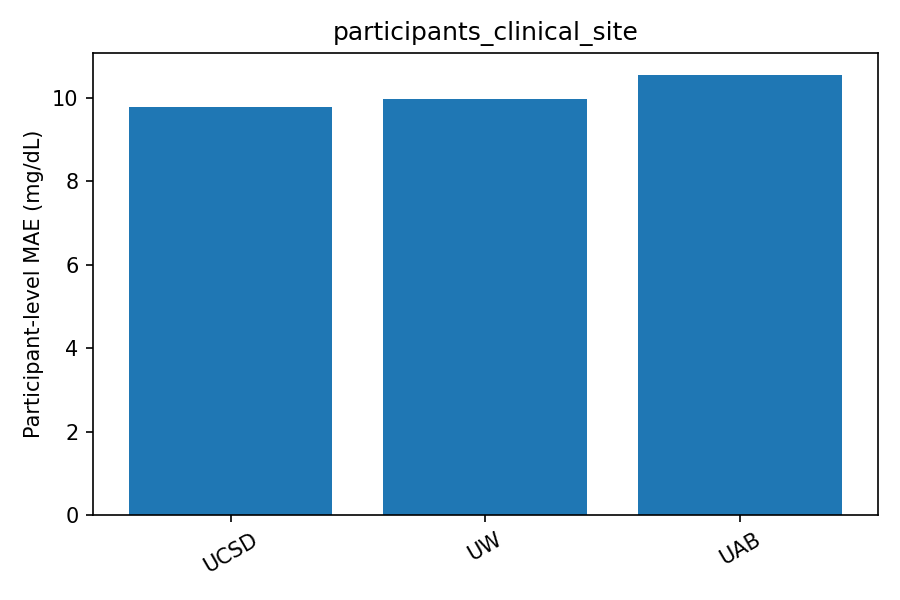
\includegraphics[width=0.82\linewidth]{figures/generated/subgroup_mae_site.png}
\caption{Participant-level MAE by clinical site. Site differences should be interpreted as possible domain shift or cohort-composition effects and require follow-up audits.}
\label{fig:subgroup_site}
\end{figure}
}
\providecommand{\GeneratedRuntimeFigures}{}
\renewcommand{\GeneratedRuntimeFigures}{%
\TODO{No runtime backend figure was found; runtime is summarized in Table~\ref{tab:runtime_metrics_generated}.}
}
\providecommand{\GeneratedAppendixFigures}{}
\renewcommand{\GeneratedAppendixFigures}{%
\begin{figure}[!htbp]
\centering
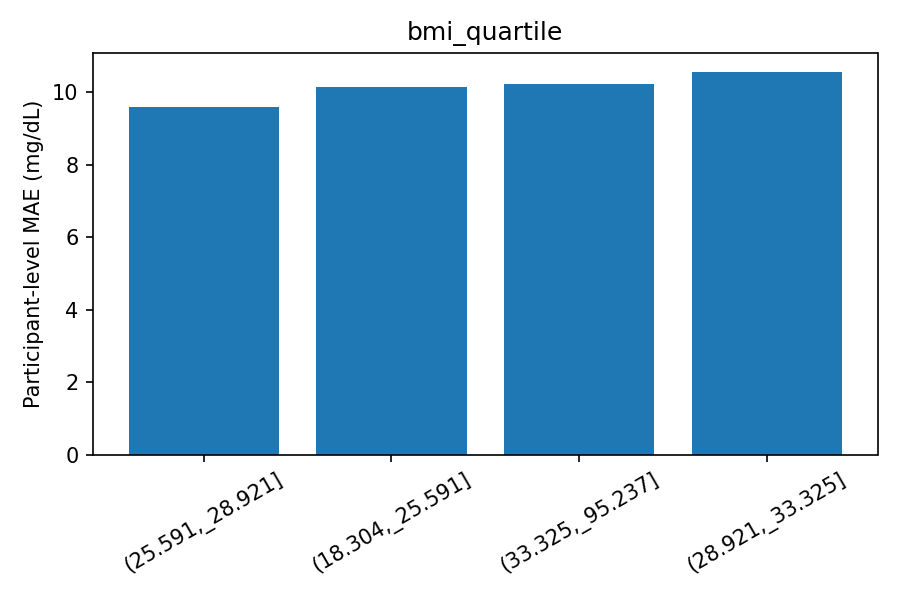
\includegraphics[width=0.82\linewidth]{figures/generated/subgroup_mae_bmi.png}
\caption{Appendix subgroup plot: participant-level MAE by BMI quartile.}
\label{fig:subgroup_bmi}
\end{figure}
\begin{figure}[!htbp]
\centering
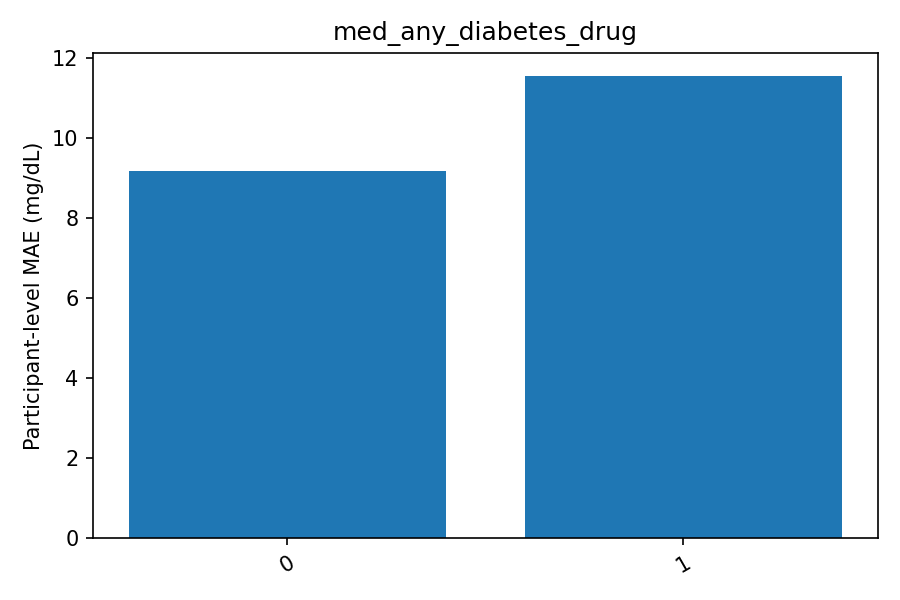
\includegraphics[width=0.82\linewidth]{figures/generated/subgroup_mae_med_any_diabetes_drug.png}
\caption{Appendix subgroup plot: participant-level MAE by any diabetes-drug metadata flag.}
\label{fig:subgroup_med_any_diabetes_drug}
\end{figure}
}
